\chapter{Analytische Geometrie}

\section{Vektorrechnung}
\begin{flushleft}
Ein Vektor kann als die Verschiebung eines Punktes gesehen werden.
Dabei kann jedoch ein einzelner Vektor auf eine beliebige Menge von Punkten angewandt werden.
Wenn man den Vektor $\vec{a}$ auf den Punkt $P$ anwendet, bekommt man also einen zweiten Punkt $P'$,
dessen Koordinaten um die Werte des Vektors $\vec{a}$ verschoben wurden.

\begin{align}
    \vec{a} &= \begin{pmatrix} 1 \\ 1 \\ 1 \end{pmatrix} \\
    P &= \left(1,2,3\right) \\
    P' &= \left(1+1,2+1,3+1\right) = \left(2,3,4\right)
\end{align}
\end{flushleft}

\begin{center}
\begin{tikzpicture}
\begin{axis}[
    view={35}{15},
    axis lines=center,
    width=15cm,height=15cm,
    xtick={1,2,3,4,5},ytick={1,2,3,4,5},ztick={1,2,3,4,5},
    xmin=0,xmax=5,ymin=0,ymax=5,zmin=0,zmax=5,
    xlabel={$x$},ylabel={$y$},zlabel={$z$}
]

\addplot3 [only marks] coordinates {(1,2,3) (2,3,4)};
\addplot3 [no marks,densely dashed] coordinates {(1,0,0) (1,2,0) (1,2,3) (1,2,0) (0,2,0)};
\addplot3 [no marks,densely dashed] coordinates {(2,0,0) (2,3,0) (2,3,4) (2,3,0) (0,3,0)};

\node [above left] at (axis cs:1,2,3) {$P(1,2,3)$};
\node [above right] at (axis cs:2,3,4) {$P'(2,3,4)$};
\draw [->,thick] (axis cs:1,2,3) to (axis cs:1.97,2.97,3.97);
\node [above left] at (axis cs:1.5,2.5,3.5) {$\vec{a}$};

\end{axis}
\end{tikzpicture}
\end{center}

\subsection{Ortsvektoren}
\begin{flushleft}   
Ortsvektoren verschieben den Ursprung des Koordinatensystems.
Der Ortsvektor $\overrightarrow{OP}$ hat also die gleichen Koordinaten, wie der Punkt $P$,
da $O=(0,0,0)$ ist.

\begin{align}
    O &= (0,0,0) \\
    P &= (1,2,3) \\
    \overrightarrow{OP} &= \begin{pmatrix} 1 \\ 2 \\ 3 \end{pmatrix}
\end{align}
\end{flushleft}

\begin{center}
\begin{tikzpicture}
\begin{axis}[
    view={35}{15},
    axis lines=center,
    width=15cm,height=15cm,
    xtick={1,2,3,4,5},ytick={1,2,3,4,5},ztick={1,2,3,4,5},
    xmin=-2,xmax=5,ymin=-2,ymax=5,zmin=-2,zmax=5,
    xlabel={$x$},ylabel={$y$},zlabel={$z$}
]

\addplot3 [only marks] coordinates {(0,0,0) (1,2,3)};
\addplot3 [no marks,densely dashed] coordinates {(1,0,0) (1,2,0) (1,2,3)};
\addplot3 [no marks,densely dashed] coordinates {(0,2,0) (1,2,0)};

\node [above right] at (axis cs:1,2,3) {$P(1,2,3)$};
\node [left] at (axis cs:0,0,0) {$O(0,0,0)$};
\draw [->,thick] (axis cs:0,0,0) to (axis cs:0.95,1.95,2.95);
\node [below] at (axis cs:0.3,1.3,2.3) {$\overrightarrow{OP}$};

\end{axis}
\end{tikzpicture}
\end{center}

\subsection{Addition}
\begin{flushleft}
Die Addition von Vektoren ist sehr simpel.
Wenn $\vec{a}$ und $\vec{b}$ addiert werden sollen, werden alle Einträge von $\vec{b}$
zu den Einträgen von $\vec{a}$ addiert.
\begin{align}
    \vec{a} &= \begin{pmatrix} 1 \\ 1 \\ 1 \end{pmatrix} \\
    \vec{b} &= \begin{pmatrix} 2 \\ 3 \\ 4 \end{pmatrix} \\
    \vec{a}+\vec{b} &= \begin{pmatrix} 1+2 \\ 1+3 \\ 1+4 \end{pmatrix} \\
    \vec{a}+\vec{b} &= \begin{pmatrix} 3 \\ 4 \\ 5 \end{pmatrix}
\end{align}
\end{flushleft}

\begin{center}
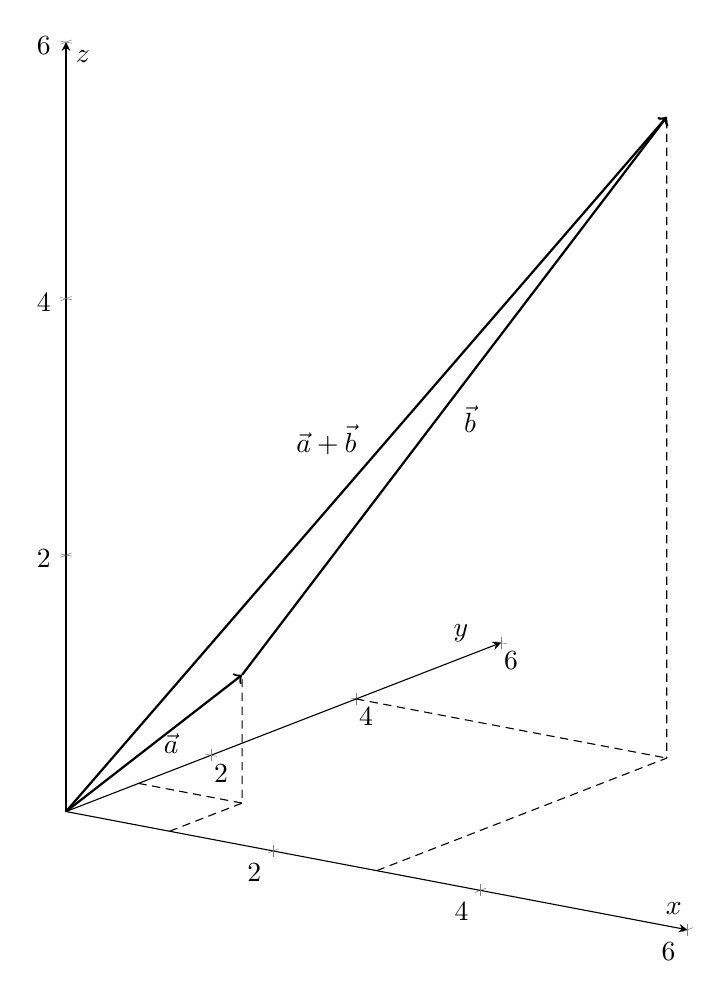
\begin{tikzpicture}
\begin{axis}[
    view={35}{15},
    axis lines=center,
    width=15cm,height=15cm,
    xtick={2,4,6},ytick={2,4,6},ztick={2,4,6},
    xmin=0,xmax=6,ymin=0,ymax=6,zmin=0,zmax=6,
    xlabel={$x$},ylabel={$y$},zlabel={$z$}
]

\addplot3 [no marks,densely dashed] coordinates {(1,0,0) (1,1,0) (1,1,1)};
\addplot3 [no marks,densely dashed] coordinates {(0,1,0) (1,1,0)};

\addplot3 [no marks,densely dashed] coordinates {(3,0,0) (3,4,0) (3,4,5)};
\addplot3 [no marks,densely dashed] coordinates {(0,4,0) (3,4,0)};

\draw [->,thick] (axis cs:0,0,0) to (axis cs:1,1,1);
\node [right] at (axis cs:0.5,0.5,0.5) {$\vec{a}$};

\draw [->,thick] (axis cs:1,1,1) to (axis cs:3,4,5);
\node [below right] at (axis cs:2,2.5,3) {$\vec{b}$};

\draw [->,thick] (axis cs:0,0,0) to (axis cs:3,4,5);
\node [above left] at (axis cs:1.5,2,2.5) {$\vec{a}+\vec{b}$};

\end{axis}
\end{tikzpicture}
\end{center}

\subsection{Multiplikation}
\begin{flushleft}    
Ein Vektor kann mit einer Zahl $r \in \mathbb{R}$ multipliziert werden.
Ähnlich wie bei der Addition werden hier alle Einträge eines Vektors mit $r$ multipliziert.

\begin{align}
    \vec{a} &= \begin{pmatrix} 1 \\ 2 \\ 3 \end{pmatrix} \\
    r &= 2 \\
    2\vec{a} &= \begin{pmatrix} 2 \cdot 1 \\ 2 \cdot 2 \\ 2 \cdot 3 \end{pmatrix} = \begin{pmatrix} 2 \\ 4 \\ 6 \end{pmatrix}
\end{align}
\end{flushleft}

\begin{center}
\begin{tikzpicture}
\begin{axis}[
    view={35}{15},
    axis lines=center,
    width=15cm,height=15cm,
    xtick={2,4,6},ytick={2,4,6},ztick={2,4,6},
    xmin=0,xmax=6,ymin=0,ymax=6,zmin=0,zmax=6,
    xlabel={$x$},ylabel={$y$},zlabel={$z$}
]

\addplot3 [no marks,densely dashed] coordinates {(1,0,0) (1,2,0) (1,2,3)};
\addplot3 [no marks,densely dashed] coordinates {(0,2,0) (1,2,0)};

\addplot3 [no marks,densely dashed] coordinates {(2,0,0) (2,4,0) (2,4,6)};
\addplot3 [no marks,densely dashed] coordinates {(0,4,0) (2,4,0)};

\draw [->,thick,red] (axis cs:1,2,3) to (axis cs:2,4,6);
\node [below right] at (axis cs:1.5,3,4.5) {$2\vec{a}$};

\draw [->,thick,blue] (axis cs:0,0,0) to (axis cs:1,2,3);
\node [right] at (axis cs:0.5,1,1.5) {$\vec{a}$};

\end{axis}
\end{tikzpicture}
\end{center}

\begin{flushleft}
Der Vektor $\vec{a}$ wird hier um $r$ verlängert.
In diesem Beispiel wird $\vec{a}$ also doppelt so lang, da $r=2$ ist.
Falls $\left| r \right| < 1$ ist, wird der Vektor $\vec{a}$ also verkürzt.

\begin{align}
    \vec{a} &= \begin{pmatrix} 1 \\ 2 \\ 3 \end{pmatrix} \\
    r &= \frac{1}{2} \\
    \frac{1}{2} \vec{a} &= \begin{pmatrix} \frac{1}{2} \cdot 1 \\ \frac{1}{2} \cdot 2 \\ \frac{1}{2} \cdot 3 \end{pmatrix} = \begin{pmatrix} \frac{1}{2} \\ 1 \\ \frac{3}{2} \end{pmatrix}
\end{align}
\end{flushleft}

\begin{center}
\begin{tikzpicture}
\begin{axis}[
    view={35}{15},
    axis lines=center,
    width=15cm,height=15cm,
    xtick={2,4,6},ytick={2,4,6},ztick={2,4,6},
    xmin=0,xmax=6,ymin=0,ymax=6,zmin=0,zmax=6,
    xlabel={$x$},ylabel={$y$},zlabel={$z$}
]

\addplot3 [no marks,densely dashed] coordinates {(1,0,0) (1,2,0) (1,2,3)};
\addplot3 [no marks,densely dashed] coordinates {(0,2,0) (1,2,0)};

\addplot3 [no marks,densely dashed] coordinates {(0.5,0,0) (0.5,1,0) (0.5,1,1.5)};
\addplot3 [no marks,densely dashed] coordinates {(0,1,0) (0.5,1,0)};

\draw [->,thick,blue] (axis cs:0,0,0) to (axis cs:0.5,1,1.5);
\node [right] at (axis cs:0.25,0.5,0.75) {$\frac{1}{2}\vec{a}$};

\draw [->,thick,red] (axis cs:0.5,1,1.5) to (axis cs:1,2,3);
\node [below right] at (axis cs:0.75,1.5,2.25) {$\vec{a}$};

\end{axis}
\end{tikzpicture}
\end{center}

\begin{flushleft}
Nach dem selben Prinzip wird die Richtung von $\vec{a}$ getauscht, wenn $r < 0$ ist.
\end{flushleft}

\begin{center}
\begin{tikzpicture}
\begin{axis}[
    view={35}{15},
    axis lines=center,
    width=15cm,height=15cm,
    xtick={1,2,3,4},ytick={1,2,3,4},ztick={1,2,3,4},
    xmin=0,xmax=4,ymin=0,ymax=4,zmin=0,zmax=4,
    xlabel={$x$},ylabel={$y$},zlabel={$z$}
]

\addplot3 [no marks,densely dashed] coordinates {(1,0,0) (1,2,0) (1,2,3)};
\addplot3 [no marks,densely dashed] coordinates {(0,2,0) (1,2,0)};

\addplot3 [no marks,densely dashed] coordinates {(0.5,0,0) (0.5,1,0) (0.5,1,1.5)};
\addplot3 [no marks,densely dashed] coordinates {(0,1,0) (0.5,1,0)};

\draw [->,thick,red] (axis cs:0,0,0) to (axis cs:1,2,3);
\node [below right,red] at (axis cs:0.25,0.5,0.75) {$\vec{a}$};

\draw [->,thick,blue] (axis cs:1,2,3) to (axis cs:0.5,1,1.5);
\node [right,blue] at (axis cs:0.75,1.5,2.25) {$\frac{-1}{2}\vec{a}$};

\end{axis}
\end{tikzpicture}
\end{center}

\begin{flushleft}
Wenn $\vec{a}$ mit $-1$ multipliziert wird, entsteht sein Gegenvektor $-\vec{a}$,
der die gleiche länge wie $\vec{a}$ hat aber in die andere Richtung zeigt.
\end{flushleft}

\begin{center}
\begin{tikzpicture}
\begin{axis}[
    view={35}{15},
    axis lines=center,
    width=15cm,height=15cm,
    xtick={1,2,3,4},ytick={1,2,3,4},ztick={1,2,3,4},
    xmin=0,xmax=4,ymin=0,ymax=4,zmin=0,zmax=4,
    xlabel={$x$},ylabel={$y$},zlabel={$z$}
]

\addplot3 [no marks,densely dashed] coordinates {(1,0,0) (1,2,0) (1,2,3)};
\addplot3 [no marks,densely dashed] coordinates {(0,2,0) (1,2,0)};

\draw [->,thick,red] (axis cs:0,0,0) to (axis cs:1,2,3);
\node [below right,red] at (axis cs:0.5,1,1.5) {$\vec{a}$};

\draw [->,thick,blue] (axis cs:1,2,3) to (axis cs:0,0,0);
\node [above left,blue] at (axis cs:0.5,1,1.5) {$-\vec{a}$};

\end{axis}
\end{tikzpicture}
\end{center}

\subsection{Subtraktion}
\begin{flushleft}
Die Subtraktion zweier Vektoren ist die Addition des einen Vektor mit dem Gegenvektor des anderen.
Es gilt also:

\begin{align}
    \vec{a} &= \begin{pmatrix} 1 \\ 1 \\ 1 \end{pmatrix} \\
    \vec{b} &= \begin{pmatrix} 2 \\ 3 \\ 4 \end{pmatrix} \\
    \vec{a}-\vec{b} &= \vec{a}+\left(-\vec{b}\right) \\
    \vec{a}-\vec{b} &= \begin{pmatrix} 1 \\ 1 \\ 1 \end{pmatrix}+\left[\begin{pmatrix}-2 \\ -3 \\ -4\end{pmatrix}\right] \\
    \vec{a}-\vec{b} &= \begin{pmatrix} -1 \\ -2 \\ -3 \end{pmatrix}
\end{align}
\end{flushleft}

\subsection{Skalarprodukt}
\begin{flushleft}
Allgemein geht es beim Skalarprodukt um die Multiplikation zweier Vektoren.

Es gilt:
\begin{align}
    \vec{a}\cdot\vec{b}=\begin{pmatrix} a_1 \\ a_2 \\ a_3 \end{pmatrix}\cdot\begin{pmatrix} b_1 \\ b_2 \\ b_3 \end{pmatrix}=a_1 b_1+a_2 b_2+a_3 b_3
\end{align}

Das Skalarprodukt zweier Vektoren ist auch nützlich um herauszufinden ob diese Vektoren zueinander
orthogonal sind.

Ein Vektor $\vec{a}$ ist nämlich orthogonal zu einem anderen Vektor $\vec{b}$, wenn:
\begin{align}
    \vec{a}\cdot\vec{b}=0
\end{align}
ist.
\end{flushleft}

\subsubsection{Herleitung}
\begin{flushleft}
Damit $\vec{a}\perp\vec{b}$ gilt, kann man $\vec{a}$ und $\vec{b}$ als Katheten eines rechtwinkligen Dreiecks sehen.
Somit ergibt sich für die Hypotenuse $\vec{b}-\vec{a}$.
Wenn jetzt der Satz des Pythagoras gilt, gilt auch $\vec{a}\perp\vec{b}$.
Konkret bedeutet das so viel:
\begin{align}
    \vec{a}&\perp\vec{b} \\
    |\vec{a}|^2+|\vec{b}|^2&=|\vec{b}-\vec{a}|^2
\end{align}

Für den ersten Teil der Gleichung ergibt sich so:
\begin{align}
    a_1^2+a_2^2+a_3^2+b_1^2+b_2^2+b_3^2
\end{align}

Der zweite Teil sieht so aus:
\begin{align}
    &\left(b_1-a_1\right)^2+\left(b_2-a_2\right)^2+\left(b_3-a_3\right)^2 \\
    \Leftrightarrow &b_1^2-2b_1a_1+a_1^2+b_2^2-2b_2a_2+a_2^2+b_3^2-2b_3a_3+a_3^2
\end{align}

Hier sieht man relativ klar, dass der erste Term nur gleich dem zweiten sein kann, wenn:
\begin{align}
    -2b_1a_1-2b_2a_2-2b_3a_3=0
\end{align}
ist, da der erste Term im zweiten enthalten ist:
\begin{align}
    \mathbf{b_1^2}-2b_1a_1+\mathbf{a_1^2}+\mathbf{b_2^2}-2b_2a_2+\mathbf{a_2^2}+\mathbf{b_3^2}-2b_3a_3+\mathbf{a_3^2}
\end{align}

Umgeformt sieht das ganze so aus:
\begin{align}
    a_1b_1+a_2b_2+a_3b_3=0
\end{align}

Deswegen gilt also:
\begin{align}
    \vec{a}\cdot\vec{b}=\begin{pmatrix} a_1 \\ a_2 \\ a_3 \end{pmatrix}\cdot\begin{pmatrix} b_1 \\ b_2 \\ b_3 \end{pmatrix}=a_1 b_1+a_2 b_2+a_3 b_3
\end{align}
\end{flushleft}

\subsubsection{Winkel zwischen Vektoren}
\begin{flushleft}
Um den Winkel $\theta$ zwischen $\vec{a}$ und $\vec{b}$ zu berechnen benötigt man die folgende Formel:
\begin{align}
    \cos\theta = \frac{\vec{a}\cdot\vec{b}}{|\vec{a}||\vec{b}|}
\end{align}

% TODO: Herleitung, welcher Winkel wird berechnet?
\end{flushleft}

\subsection{Geraden im Raum}
\begin{flushleft}
Eine Gerade $g$ im Raum besteht aus einem Stützvektor $\vec{v}$ und einem Richtungsvektor $\vec{r}$.

\begin{align}
    g\colon\vec{x}=\vec{v}+t\cdot\vec{r}
\end{align}
\end{flushleft}

% TODO: Geradengleichungen aufstellen

\subsubsection{Punkte einer Geraden bestimmen}
\begin{flushleft}
Beispielhaft ist hier die Gerade $g$ wie folgt definiert:
\begin{align}
    g\colon\vec{x}=\begin{pmatrix} 1 \\ 1 \\ 1 \end{pmatrix}+t\cdot\begin{pmatrix} 1 \\ 1 \\ 1 \end{pmatrix}
\end{align}

Um verschiedene Punkte zu bestimmen, die auf der Geraden liegen muss man bloß einen Wert für $t$ einsetzen:
\begin{align}
    \vec{x}_0=\begin{pmatrix} 1 \\ 1 \\ 1 \end{pmatrix}+0\cdot\begin{pmatrix} 1 \\ 1 \\ 1 \end{pmatrix}=\begin{pmatrix} 1 \\ 1 \\ 1 \end{pmatrix} \\
    \vec{x}_1=\begin{pmatrix} 1 \\ 1 \\ 1 \end{pmatrix}+1\cdot\begin{pmatrix} 1 \\ 1 \\ 1 \end{pmatrix}=\begin{pmatrix} 2 \\ 2 \\ 2 \end{pmatrix}
\end{align}
\end{flushleft}

\subsubsection{Punktproben}
\begin{flushleft}
Wenn man prüfen möchte ob der Punkt $P(1|1|1)$ auf der Geraden:
\begin{align}
    g\colon\vec{x}=\begin{pmatrix} 1 \\ 1 \\ 1 \end{pmatrix}+t\cdot\begin{pmatrix} 1 \\ 1 \\ 1 \end{pmatrix}
\end{align}
liegt, setzt man den Ortsvektor des Punktes $P$ in die Gerade $g$ ein:
\begin{align}
    \begin{pmatrix} 1 \\ 1 \\ 1 \end{pmatrix}=\begin{pmatrix} 1 \\ 1 \\ 1 \end{pmatrix}+t\cdot\begin{pmatrix} 1 \\ 1 \\ 1 \end{pmatrix}
\end{align}

Hier wird schnell klar, dass der Punkt $P(1|1|1)$ für $t=0$ auf der Geraden $g$ liegt, da der Richtungsvektor für $t=0$ wegfällt und der Stützvektor und der Ortsvektor zum Punkt $P$ identisch sind.

Der allgemeine Lösungsansatz ist jedoch ein Gleichungsystem zu bilden:
\begin{align}
    1&=1+t \label{eins} \\
    1&=1+t \label{zwei} \\
    1&=1+t \label{drei}
\end{align}
Das LGS besteht aus den drei Gleichungen \eqref{eins}, \eqref{zwei} und \eqref{drei}.
Da alle Gleichungen identisch sind, reicht es hier eine beliebige Gleichung nach $t$ aufzulösen:
\begin{align}
    1&=1+t \\
    \Leftrightarrow 0&=t
\end{align}
Dieser Lösungsweg zeigt auch, dass der Punkt $P(1|1|1)$ für $t=0$ auf der Geraden $g$ liegt.
\end{flushleft}

\subsubsection{Orthogonalität}
\begin{flushleft}
Möchte man eine Gerade $h$ finden, die zu einer anderen Geraden $g$ orthogonal verläuft, müssen die Richtungsvektoren beider Geraden orthogonal zueinander sein.

Um eine Gerade zu finden, die orthogonal zu der Geraden:
\begin{align}
    g\colon\vec{x}=\begin{pmatrix} 1 \\ 1 \\ 1 \end{pmatrix}+t\cdot\begin{pmatrix} 1 \\ 1 \\ 1 \end{pmatrix}
\end{align}
verläuft, muss man einen Vektor $\vec{r_h}$ finden, der orthogonal zu dem Richtungsvektor $\vec{r_g}$ von $g$ ist:
\begin{align}
    \vec{r_h}&\perp\vec{r_g} \\
    \Leftrightarrow \vec{r_h}\cdot\vec{r_g}&=0 \\
    \Leftrightarrow \begin{pmatrix} r_1 \\ r_2 \\ r_3 \end{pmatrix}\cdot\begin{pmatrix} 1 \\ 1 \\ 1 \end{pmatrix}&=0 \\
    \Leftrightarrow r_1+r_2+r_3&=0 \\
    \Leftrightarrow r_1&=-r_2-r_3 \\
    \Leftrightarrow r_2&=-r_1-r_3 \\
    \Leftrightarrow r_3&=-r_1-r_2
\end{align}
Nun hat man eine Gleichung mit drei Unbekannten, deshalb kann man zwei dieser Unbekannten frei wählen, wählt man also $r_1=1$ und $r_2=2$ ergibt sich die folgende Gleichung für $h$:
\begin{align}
    r_1&=1 \\
    r_2&=2 \\
    r_3&=-1-2=-3 \\
    \vec{r_h}&=\begin{pmatrix} 1 \\ 2 \\ -3 \end{pmatrix} \\
    h\colon\vec{x}&=\begin{pmatrix} 1 \\ 1 \\ 1 \end{pmatrix}+s\cdot\begin{pmatrix} 1 \\ 2 \\ -3 \end{pmatrix}
\end{align}
\end{flushleft}

\subsection{Ebenen im Raum}
\begin{flushleft}
Eine Ebene im Raum kann durch verschiedene Formen dargestellt werden.
Man unterscheidet zwischen Parameter-, Normalen-, und Koordinatenform.
\end{flushleft}

\subsubsection{Parameterform}
\begin{flushleft}
Eine Ebene $E$ in der Parameterform hat einen Stützvektor $\vec{s}$ und zwei Spannvektoren $\vec{u}$ und $\vec{v}$, die keine Vielfachen von einander sind:
\begin{align}
    E\colon\vec{x}=\vec{s}+t\vec{u}+s\vec{v} \quad t,s\in\mathbb{R}
\end{align}
\end{flushleft}

% TODO: Ebenengleichungen aufstellen

\subsubsection{Normalenform}
\begin{flushleft}
Eine Ebene $E$ in der Normalenform besteht aus einem Normalenvektor $\vec{n}$, der senkrecht zur Ebene steht, und einem Stützvektor $\vec{p}$:
\begin{align}
    E\colon\vec{n}\cdot\left(\vec{x}-\vec{p}\right)=0
\end{align}
\end{flushleft}

% TODO: Normalen-, Koordinatengleichungen aufstellen

\subsubsection{Koordinatenform}
\begin{flushleft}
Die Koordinatenform ist eine Erweiterung der Normalenform:
\begin{align}
    \vec{n}\cdot\left(\vec{x}-\vec{p}\right)&=0 \\
    \Leftrightarrow \vec{n}\cdot\vec{x}-\vec{n}\cdot\vec{p}&=0 \\
    \Leftrightarrow \vec{n}\cdot\vec{x}&=\vec{n}\cdot\vec{p} \\
    \Leftrightarrow \begin{pmatrix}n_1 \\ n_2 \\ n_3 \end{pmatrix}\cdot\begin{pmatrix}x_1 \\ x_2 \\ x_3 \end{pmatrix}&=\vec{n}\cdot\vec{p} \\
    \Leftrightarrow n_1x_1+n_2x_2+n_3x_3&=d \quad n_1,n_2,n_3,d\in\mathbb{R}
\end{align}

Eine Ebene $E$ in der Koordinatenform besteht also aus den Koordinaten $n_1, n_2, n_3$ des Normalenvektors $\vec{n}$ und dem Wert $d$, der sich aus $\vec{n}\cdot\vec{p}$ ergibt:
\begin{align}
    E\colon n_1x_1+n_2x_2+n_3x_3&=d \quad n_1,n_2,n_3,d\in\mathbb{R}
\end{align}
\end{flushleft}

\subsection{Schnittpunkte zwischen Geraden}
\begin{flushleft}
Die Schnittpunkte zwischen einer Geraden $g$ und einer anderen Geraden $h$ kann man herausfinden indem man beide Geraden gleichsetzt.
\begin{align}
    g\colon\vec{x}&=\begin{pmatrix} 1 \\ 1 \\ 1 \end{pmatrix}+t\begin{pmatrix} 1 \\ 1 \\ 1 \end{pmatrix} \\
    h\colon\vec{x}&=\begin{pmatrix} 1 \\ 1 \\ 1 \end{pmatrix}+s\begin{pmatrix} 1 \\ 2 \\ 1 \end{pmatrix} \\
    g&=h \\
    \begin{pmatrix} 1 \\ 1 \\ 1 \end{pmatrix}+t\begin{pmatrix} 1 \\ 1 \\ 1 \end{pmatrix}&=\begin{pmatrix} 1 \\ 1 \\ 1 \end{pmatrix}+s\begin{pmatrix} 1 \\ 2 \\ 1 \end{pmatrix}
\end{align}

Aus den Koordinaten $x_1,x_2,x_3$ ergibt sich ein lineares Gleichungssystem aus drei Gleichungen:
\begin{align}
    \text{I}\colon& 1+t=1+s \\
    \text{II}\colon& 1+t=1+2s \\
    \text{III}\colon& 1+t=1+s
\end{align}

Nun muss das LGS gelöst werden ($III$ wurde entfernt, da $I$=$III$):
\begin{align}
    \text{I}\colon& 1+t=1+s \\
    \text{II}\colon& 1+t=1+2s \\
    \text{Schritt 1}& \\
    \text{I}'\colon& t=s \\
    \text{II}\colon& 1+t=1+2s \\
    \text{Schritt 2}& \\
    \text{I}'\colon& t=s \\
    \text{II}'\colon& 1+s=1+2s \\
    \text{Schritt 3}& \\
    \text{I}'\colon& t=s \\
    \text{II}''\colon& 1=1+s \\
    \text{Schritt 4}& \\
    \text{I}'\colon& t=s \\
    \text{II}'''\colon& 0=s \\
    \text{Lösung}& \\
    &t=s=0
\end{align}

Hier ist der einzige Schnittpunkt der Stützvektor zum Punkt $S(1|1|1)$ beider Geraden.

Zwei Geraden können:
\begin{enumerate}
    \item {windschief verlaufen,}
    \item {parallel verlaufen,}
    \item {einen Schnittpunkt haben.}
\end{enumerate}
\end{flushleft}

\subsection{Schnittpunkte zwischen Gerade und Ebene}
\subsubsection{Ebene in Parameterform}
\begin{flushleft}
Liegt eine Ebene in Parameterform vor, können Gerade und Ebene gleichgesetzt werden.
Beispielsweise kann man die Gerade $g$ gleich der Ebene $E$ setzen:
\begin{align}
    g\colon\vec{x}&=\begin{pmatrix} 1 \\ 1 \\ 1 \end{pmatrix}+t\begin{pmatrix} 1 \\ 1 \\ 1 \end{pmatrix} \\
    E\colon\vec{x}&=\begin{pmatrix} 1 \\ 1 \\ 1 \end{pmatrix}+r\begin{pmatrix} 2 \\ 1 \\ 1 \end{pmatrix}+s\begin{pmatrix} 1 \\ 2 \\ 1 \end{pmatrix} \\
    \begin{pmatrix} 1 \\ 1 \\ 1 \end{pmatrix}+t\begin{pmatrix} 1 \\ 1 \\ 1 \end{pmatrix}&=\begin{pmatrix} 1 \\ 1 \\ 1 \end{pmatrix}+r\begin{pmatrix} 2 \\ 1 \\ 1 \end{pmatrix}+s\begin{pmatrix} 1 \\ 2 \\ 1 \end{pmatrix} \\
    \text{I}\colon& 1+t=1+2r+s \\
    \text{II}\colon& 1+t=1+r+2s \\
    \text{III}\colon& 1+t=1+r+s \\
    \text{Schritt 1}& \\
    \text{I}\colon& 1+t=1+2r+s \\
    \text{II}'\colon& 0=s \\
    \text{III}\colon& 1+t=1+r+s \\
    \text{Schritt 2}& \\
    \text{I}'\colon& 0=r \\
    \text{II}'\colon& 0=s \\
    \text{III}\colon& 1+t=1+r+s \\
    \text{Schritt 3}& \\
    \text{I}'\colon& 0=r \\
    \text{II}'\colon& 0=s \\
    \text{III}'\colon& 1+t=1 \Leftrightarrow t=0
\end{align}

Die Gerade $g$ schneidet die Ebene $E$ für $t=r=s=0$ im Punkt $S(1|1|1)$.
\end{flushleft}

\subsection{Schnittpunkte zwischen Ebenen}
% TODO: Schnittpunkte zwischen Ebenen

\section{Matrizen}
\begin{flushleft}
Matrizen sind sehr nützlich um viele verschiedene Werte in einen Kontext zu bringen.
So lassen sich beispielsweise ein- oder mehrstufige Prozesse durch Matrizen darstellen.
\end{flushleft}

\subsection{Einstufige Prozesse}
\begin{flushleft}   
Beispielsweise können durch die Mischung von Kaffepulver, Wasser und Milch unterschiedliche Kaffesorten produziert werden:
\end{flushleft}

\begin{center}
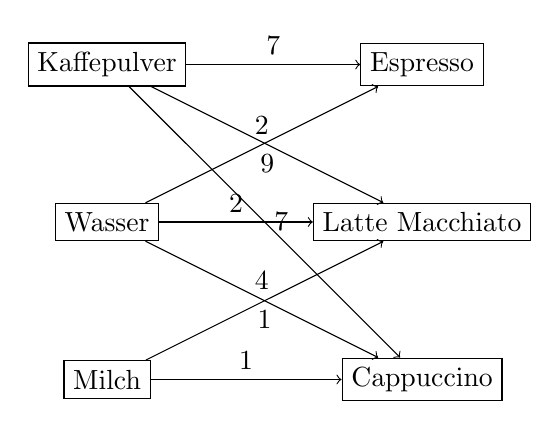
\begin{tikzpicture}
    \node[shape=rectangle,draw=black] (K) at (0,0) {Kaffepulver};
    \node[shape=rectangle,draw=black] (W) at (0,-2) {Wasser};
    \node[shape=rectangle,draw=black] (M) at (0,-4) {Milch};
    \node[shape=rectangle,draw=black] (E) at (4,0) {Espresso};
    \node[shape=rectangle,draw=black] (L) at (4,-2) {Latte Macchiato};
    \node[shape=rectangle,draw=black] (C) at (4,-4) {Cappuccino};

    \path [->] (K) edge node[above] {$7$} (E);
    \path [->] (K) edge node[below] {$9$} (L);
    \path [->] (K) edge node[above,right] {$7$} (C);
    \path [->] (W) edge node[above] {$2$} (E);
    \path [->] (W) edge node[above] {$2$} (L);
    \path [->] (W) edge node[above] {$4$} (C);
    \path [->] (M) edge node[below] {$1$} (L);
    \path [->] (M) edge node[above] {$1$} (C);
\end{tikzpicture}
\end{center}

\begin{center}
\begin{tabular}{c|c|c|c}
& Espresso & Latte Macchiato & Cappuccino \\
\hline
Kaffepulver & 7 & 9 & 7 \\
\hline
Wasser & 2 & 2 & 4 \\
\hline
Milch & 0 & 1 & 1 \\
\end{tabular}
\end{center}

\begin{flushleft}
Dieser Prozess kann durch eine Matrix $A$ dargestellt werden:
\begin{align}
    A = \begin{pmatrix}
        7 & 9 & 7 \\
        2 & 2 & 4 \\
        0 & 1 & 1
    \end{pmatrix}
\end{align}

Um den Bedarf an Kaffepulver, Wasser und Milch für 20 Tassen Espresso, 30 Tassen Latte Macchiato und 15 Tassen Cappuccino zu errechnen,
kann man nun die Matrix $A$ mit dem Vektor $\vec{r}$ multiplizieren, der die gewünschten Werte enthält,
so bekommt man einen anderen Vektor $\vec{s}$, der den Bedarf enthält:
\begin{align}
    A\cdot\vec{r}&=\vec{s} \\
    \begin{pmatrix}
        7 & 9 & 7 \\
        2 & 2 & 4 \\
        0 & 1 & 1
    \end{pmatrix}\cdot
    \begin{pmatrix}
        20 \\
        30 \\
        15
    \end{pmatrix}&=\vec{s}
\end{align}

Aber wie multipliziert man eine Matrix mit einem Vektor?
\newline

Bei einer Matrixmultiplikation sind die Formen der beiden zu multiplizierenden Matrizen zu beachten.
Grundlegend gilt, dass jeder Vektor eine Matrix ist.

Die Matrix $A$ ist hier eine Matrix der Form 3x3, also eine quadratische Matrix, da sie drei Spalten und drei Zeilen hat.
Der Vektor $\vec{r}$ ist hier eine 3x1-Matrix.

Eine Matrix ist immer dann quadratisch, wenn die Anzahl von Spalten gleich der Anzahl von Zeilen ist.

Allgemein dürfen zwei Matrizen $A$ und $B$ nur miteinander multipliziert werden, wenn die Anzahl der Spalten, der Matrix $A$, der Anzahl der Reihen der Matrix $B$ entspricht.

Schaut man sich also die Formen von $A$ und $\vec{r}$ an, sieht man, dass die inneren Werte der beiden Formen gleich sein müssen: 3x\underline{\textbf{3} \textbf{3}}x1.
\newline

Eine Matrixmultiplikation kann man vereinfacht so betrachten, dass die zweite Matrix auf die erste geklappt wird.
Dann wird für jede Zeile das Skalarprodukt gebildet:
\end{flushleft}

\begin{center}
\begin{tabular}{r|l}
& \color{red} 20 \\
& \color{green} 30 \\
& \color{blue} 15 \\
\hline
\color{red} 7 \space \color{green} 9 \space \color{blue} 7 & $7*20+9*30+7*15=515$ \\
\color{red} 2 \space \color{green} 2 \space \color{blue} 4 & $2*20+2*30+4*15=160$ \\
\color{red} 0 \space \color{green} 1 \space \color{blue} 1 & $0*20+1*30+1*15=45$
\end{tabular}
\end{center}

\begin{flushleft}
Das Ergebnis der Multiplikation ist also der Vektor $\vec{s}$:
\begin{align}
    \vec{s}=\begin{pmatrix}
        515 \\
        160 \\
        45
    \end{pmatrix}
\end{align}
\end{flushleft}

\subsection{Zweistufige Prozesse}
\begin{flushleft}
Beispielsweise können verschiedene Eissorten aus Milch $M$, Zucker $Z$ und Früchten $F$ produziert werden.
Bei der Herstellung werden jedoch erst die Zwischenprodukte $S_1$ und $S_2$ produziert, bevor die Endprodukte $E_1$ und $E_2$ produziert werden können.
\end{flushleft}

\begin{center}
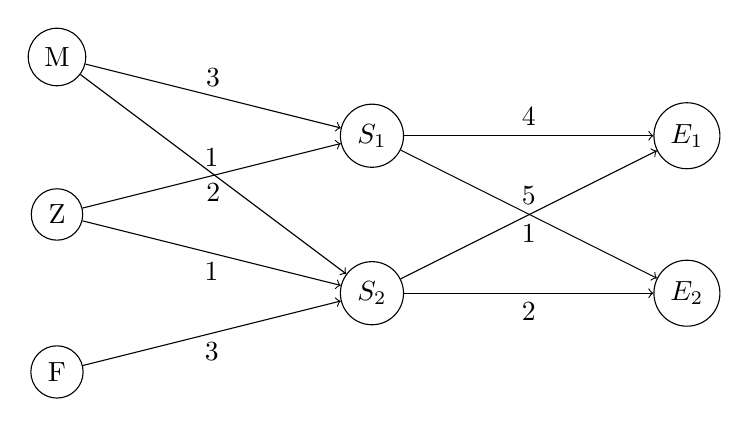
\begin{tikzpicture}
    \node[shape=circle,draw=black] (M) at (0,0) {M};
    \node[shape=circle,draw=black] (Z) at (0,-2) {Z};
    \node[shape=circle,draw=black] (F) at (0,-4) {F};
    \node[shape=circle,draw=black] (S1) at (4,-1) {$S_1$};
    \node[shape=circle,draw=black] (S2) at (4,-3) {$S_2$};
    \node[shape=circle,draw=black] (E1) at (8,-1) {$E_1$};
    \node[shape=circle,draw=black] (E2) at (8,-3) {$E_2$};

    \path [->] (M) edge node[above] {$3$} (S1);
    \path [->] (M) edge node[below] {$2$} (S2);
    \path [->] (Z) edge node[above] {$1$} (S1);
    \path [->] (Z) edge node[below] {$1$} (S2);
    \path [->] (F) edge node[below] {$3$} (S2);
    \path [->] (S1) edge node[above] {$4$} (E1);
    \path [->] (S1) edge node[above] {$5$} (E2);
    \path [->] (S2) edge node[below] {$1$} (E1);
    \path [->] (S2) edge node[below] {$2$} (E2);
\end{tikzpicture}
\end{center}

\begin{center}
\begin{tabular}{c|c|c}
& $S_1$ & $S_2$ \\
\hline
M & 3 & 2 \\
\hline
Z & 1 & 1 \\
\hline
F & 0 & 3
\end{tabular}
\end{center}

\begin{center}
\begin{tabular}{c|c|c}
& $E_1$ & $E_2$ \\
\hline
$S_1$ & 4 & 5 \\
\hline
$S_2$ & 1 & 2
\end{tabular}
\end{center}

\begin{flushleft}
Die Matrix $A$ modelliert den ersten Prozess, $B$ den zweiten:
\begin{align}
    A=\begin{pmatrix}
        3 & 2 \\
        1 & 1 \\
        0 & 3
    \end{pmatrix} \\
    B=\begin{pmatrix}
        4 & 5 \\
        1 & 2
    \end{pmatrix}
\end{align}

Um eine Ausgangsprodukt-Endprodukt Matrix $C$ zu erzeugen, muss $A$ mit $B$ multipliziert werden:
\begin{align}
    C&=A \cdot B \\
    C&=\begin{pmatrix}
        3 & 2 \\
        1 & 1 \\
        0 & 3
    \end{pmatrix} \cdot
    \begin{pmatrix}
        4 & 5 \\
        1 & 2
    \end{pmatrix} \\
    C&=\begin{pmatrix}
        14 & 19 \\
        5 & 7 \\
        3 & 6
    \end{pmatrix}
\end{align}

Die Matrix $C$ gibt an, wie viele Ausgangsprodukte notwendig sind um Endprodukte herzustellen:
\end{flushleft}

\begin{center}
\begin{tabular}{c|c|c}
& $E_1$ & $E_2$ \\
\hline
M & 14 & 19 \\
\hline
Z & 5 & 7 \\
\hline
F & 3 & 6
\end{tabular}
\end{center}

\begin{flushleft}
Wenn man nun wissen möchte, wie viele Ausgangsprodukte notwendig sind, um zum Beispiel ein mal $E_1$ und kein mal $E_2$ herzustellen, kann man die Matrix $C$ mit dem Vektor $\vec{r}$ multiplizieren, der die Anzahl der Ausgangsprodukte abbildet:
\begin{align}
    C \cdot \begin{pmatrix} 1 \\ 0 \end{pmatrix}=\begin{pmatrix} 14 \\ 5 \\ 3 \end{pmatrix}
\end{align}

Um ein mal $E_1$ und kein mal $E_2$ herzustellen braucht man also 14 Milch, 5 Zucker und 3 Früchte.
\end{flushleft}

\subsection{Inverse Matrizen}
\begin{flushleft}
Die Inverse einer Matrix $A$ ist eine andere Matrix $A^{-1}$, mit der die ursprüngliche Matrix $A$ multipliziert werden kann um die Einheitsmatrix zu bekommen.
Es gilt also:
\begin{align}
    A \cdot A^{-1}=E=A^{-1} \cdot A
\end{align}

Eine Einheitsmatrix der Form 4x4 sieht so aus:
\begin{align}
    E^4=\begin{pmatrix}
        1 & 0 & 0 & 0 \\
        0 & 1 & 0 & 0 \\
        0 & 0 & 1 & 0 \\
        0 & 0 & 0 & 1
    \end{pmatrix}
\end{align}

Wenn eine Matrix $B$ mit der Einheitsmatrix $E$ multipliziert wird, ist das Ergebnis wieder die Matrix $B$:
\begin{align}
    B \cdot E=B
\end{align}

Inverse Matrizen sind demnach sehr nützlich um Matrizengleichungen zu lösen:
\begin{align}
    A \cdot B&=C \\
    A^{-1} \cdot A \cdot B&=A^{-1} \cdot C
    \quad (A^{-1} \cdot A=E) \\
    E \cdot B&=A^{-1} \cdot C \\
    B&=A^{-1} \cdot C
\end{align}
\end{flushleft}
